\documentclass[10pt,twocolumn,letterpaper]{article}

\usepackage{cvpr}
\usepackage{times}
\usepackage{epsfig}
\usepackage{graphicx}
\usepackage{amsmath}
\usepackage{amssymb}
\usepackage{caption}
\usepackage{subcaption}
\usepackage{booktabs}
\usepackage{makecell}

% Include other packages here, before hyperref.

% If you comment hyperref and then uncomment it, you should delete
% egpaper.aux before re-running latex.  (Or just hit 'q' on the first latex
% run, let it finish, and you should be clear).
\usepackage[pagebackref=true,breaklinks=true,letterpaper=true,colorlinks,bookmarks=false]{hyperref}

%%%%%%%%% PAPER ID  - PLEASE UPDATE
\def\cvprPaperID{0947} % *** Enter the CVPR Paper ID here
\def\httilde{\mbox{\tt\raisebox{-.5ex}{\symbol{126}}}}

\begin{document}

%%%%%%%%% TITLE - PLEASE UPDATE
\title{Guided Proofreading of Automatic Segmentations for Connectomics}  % **** Enter the paper title here

\maketitle
\thispagestyle{empty}

Thank you for your constructive comments. We will fix all minor issues. We would like to clarify the following major remarks.

\section{Quantitative Evaluation}
Reviewer 2 requests an objective quantitative evaluation. We define such experiments in lines 573-590 and report the results in Fig.~6, Fig.~7 and lines 792-818 (also in supplemental Sec.~2 and 3). The evaluation is fully numeric and we report VI scores. We will change the wording in the manuscript to emphasize this.

\section{Reproducibility}
Reviewer 2 expresses concerns regarding reproducibility. However, we define all parameters in the manuscript and promise to release code and data (line 847).

\section{Optimal Parameters}
We define several parameters in the paper. However, we agree with reviewer 2 that finding the optimal values could be better explained and will synchronize this information with the paper. 
The \textbf{threshold $p_t=0.95$} was observed to be stable when evaluating on previously unseen testing data (lines 585-586, supplemental Sec. 1.3). The \textbf{input border is dilated by 5 pixels} to consider slight edge ambiguities and to cover extra-cellular space between segments in high-resolution electron microscopy data (lines 308-310). During merge error detection, \textbf{labels are dilated by 20 pixels} prior to finding potential borders (line 323) with border-seeded watershed---this way the borders tend to attach to real membrane boundaries (lines 364-366). 
%Here, we list all parameters and describe how their values are obtained. We will synchronize this information with the paper.

%
%\begin{itemize}
%\item \textbf{Threshold $p_t$.} The threshold $p_t=0.95$ was observed to be stable when evaluating on previously unseen testing data (lines 585-586, supplemental Sec. 1.3).
%\item \textbf{Dilated Boundary Input.} We dilate the border between segments by 5 pixels to consider slight edge ambiguities and to cover extra-cellular space between segments in high-resolution electron microscopy data (lines 308-310).
%\item \textbf{Dilated Label.} During merge error detection, labels are dilated by 20 pixels prior to finding potential borders (line 323) with border-seeded watershed. By doing so, the borders tend to attach to real membrane boundaries (lines 364-366).
%\end{itemize}

%\begin{table}[h]
%\caption{Parameters of GP, their values and how these values are obtained.}%While the training of our classifier is more expensive, testing accuracy is superior. }
%\resizebox{\linewidth}{!}{
%\begin{tabular}{l}
%\toprule
%Threshold $p_t=0.95$, Observed on previously unseed testing data (lines 585-586, supplemental Sec. 1.3) \\ 
%\bottomrule
%\end{tabular} 
%}
%\label{tab:parameters}
%\end{table}

\section{Training Datasets U-net vs. GP}
Reviewer 3 raises the question if GP was trained on the same data as membrane detection (U-net). There was no overlap (Tab.~\ref{tab:trainingdata}).

\begin{table}[h]
\caption{Training data of membrane detection vs. training data of GP (for supplemental material).}%While the training of our classifier is more expensive, testing accuracy is superior. }
\resizebox{\linewidth}{!}{
\begin{tabular}{lrrrr}
\toprule
Dataset & \makecell{Training Set\\Membrane Detection (U-Net)} & \makecell{Training Set\\Guided Proofreading} \\ 
\midrule
\makecell{\emph{L. Cylinder}\\~} & \makecell{AC3+AC4\\($1024\times1024\times175$vx)} & \makecell{L. Cylinder\\($2048\times2048\times250$vx)} \\ 
\makecell{\emph{AC4 subvolume}\\~} & \makecell{AC4 excl. test\\ ($1024\times1024\times90$vx)} &  \makecell{L. Cylinder\\ ($2048\times2048\times250$vx)} \\ 
\makecell{\emph{CREMI A/B/C}\\~} & \makecell{AC3+AC4\\($1024\times1024\times175$vx)} & \makecell{CREMI A/B/C\\($1250\times1250\times300$vx)} \\ 
\bottomrule
\end{tabular} 
}
\label{tab:trainingdata}
\end{table}


\section{Faster Proofreading}
We agree with reviewer 2 that our results regarding faster proofreading with GP are not clearly presented. 
%We report the average correction times for novice users in lines 756-765. Figure 7 (column 3) shows VI reduction after 30 minutes and the slopes in figure 6 also indicate better performance for GP. However, this presentation is not ideal and 
We will add Tab.~\ref{tab:correctiontimes} to the paper (previously reported in lines 756-765, slopes in figure 6, column 3 in figure 7) to better present our findings.

\begin{table}[h]
\caption{Average proofreading speed for novice users of Dojo, FP and GP. Higher VI reduction per minute shows better performance of GP.}%While the training of our classifier is more expensive, testing accuracy is superior. }
\resizebox{\linewidth}{!}{
\begin{tabular}{lrrrr}
\toprule
 & \makecell{Correction Time [s]} & \makecell{VI Reduction per minute} \\
\midrule
\emph{Dojo} & 30.5 & -0.002 \\
\emph{FP} & 4.9 & 0.00023 \\
\emph{GP} & 6.2 & 0.00173 \\
\bottomrule
\end{tabular} 
}
\label{tab:correctiontimes}
\end{table}

\section{Merge Error Detection}

Reviewer 3 suggests a better explanation of the merge error detection. We updated figure 4 in the paper to include the watershed seeds (Fig. 1). We will also add a pseudo code version of the algorithm to the supplemental material to promote understanding.

\begin{figure}[h]
\centering
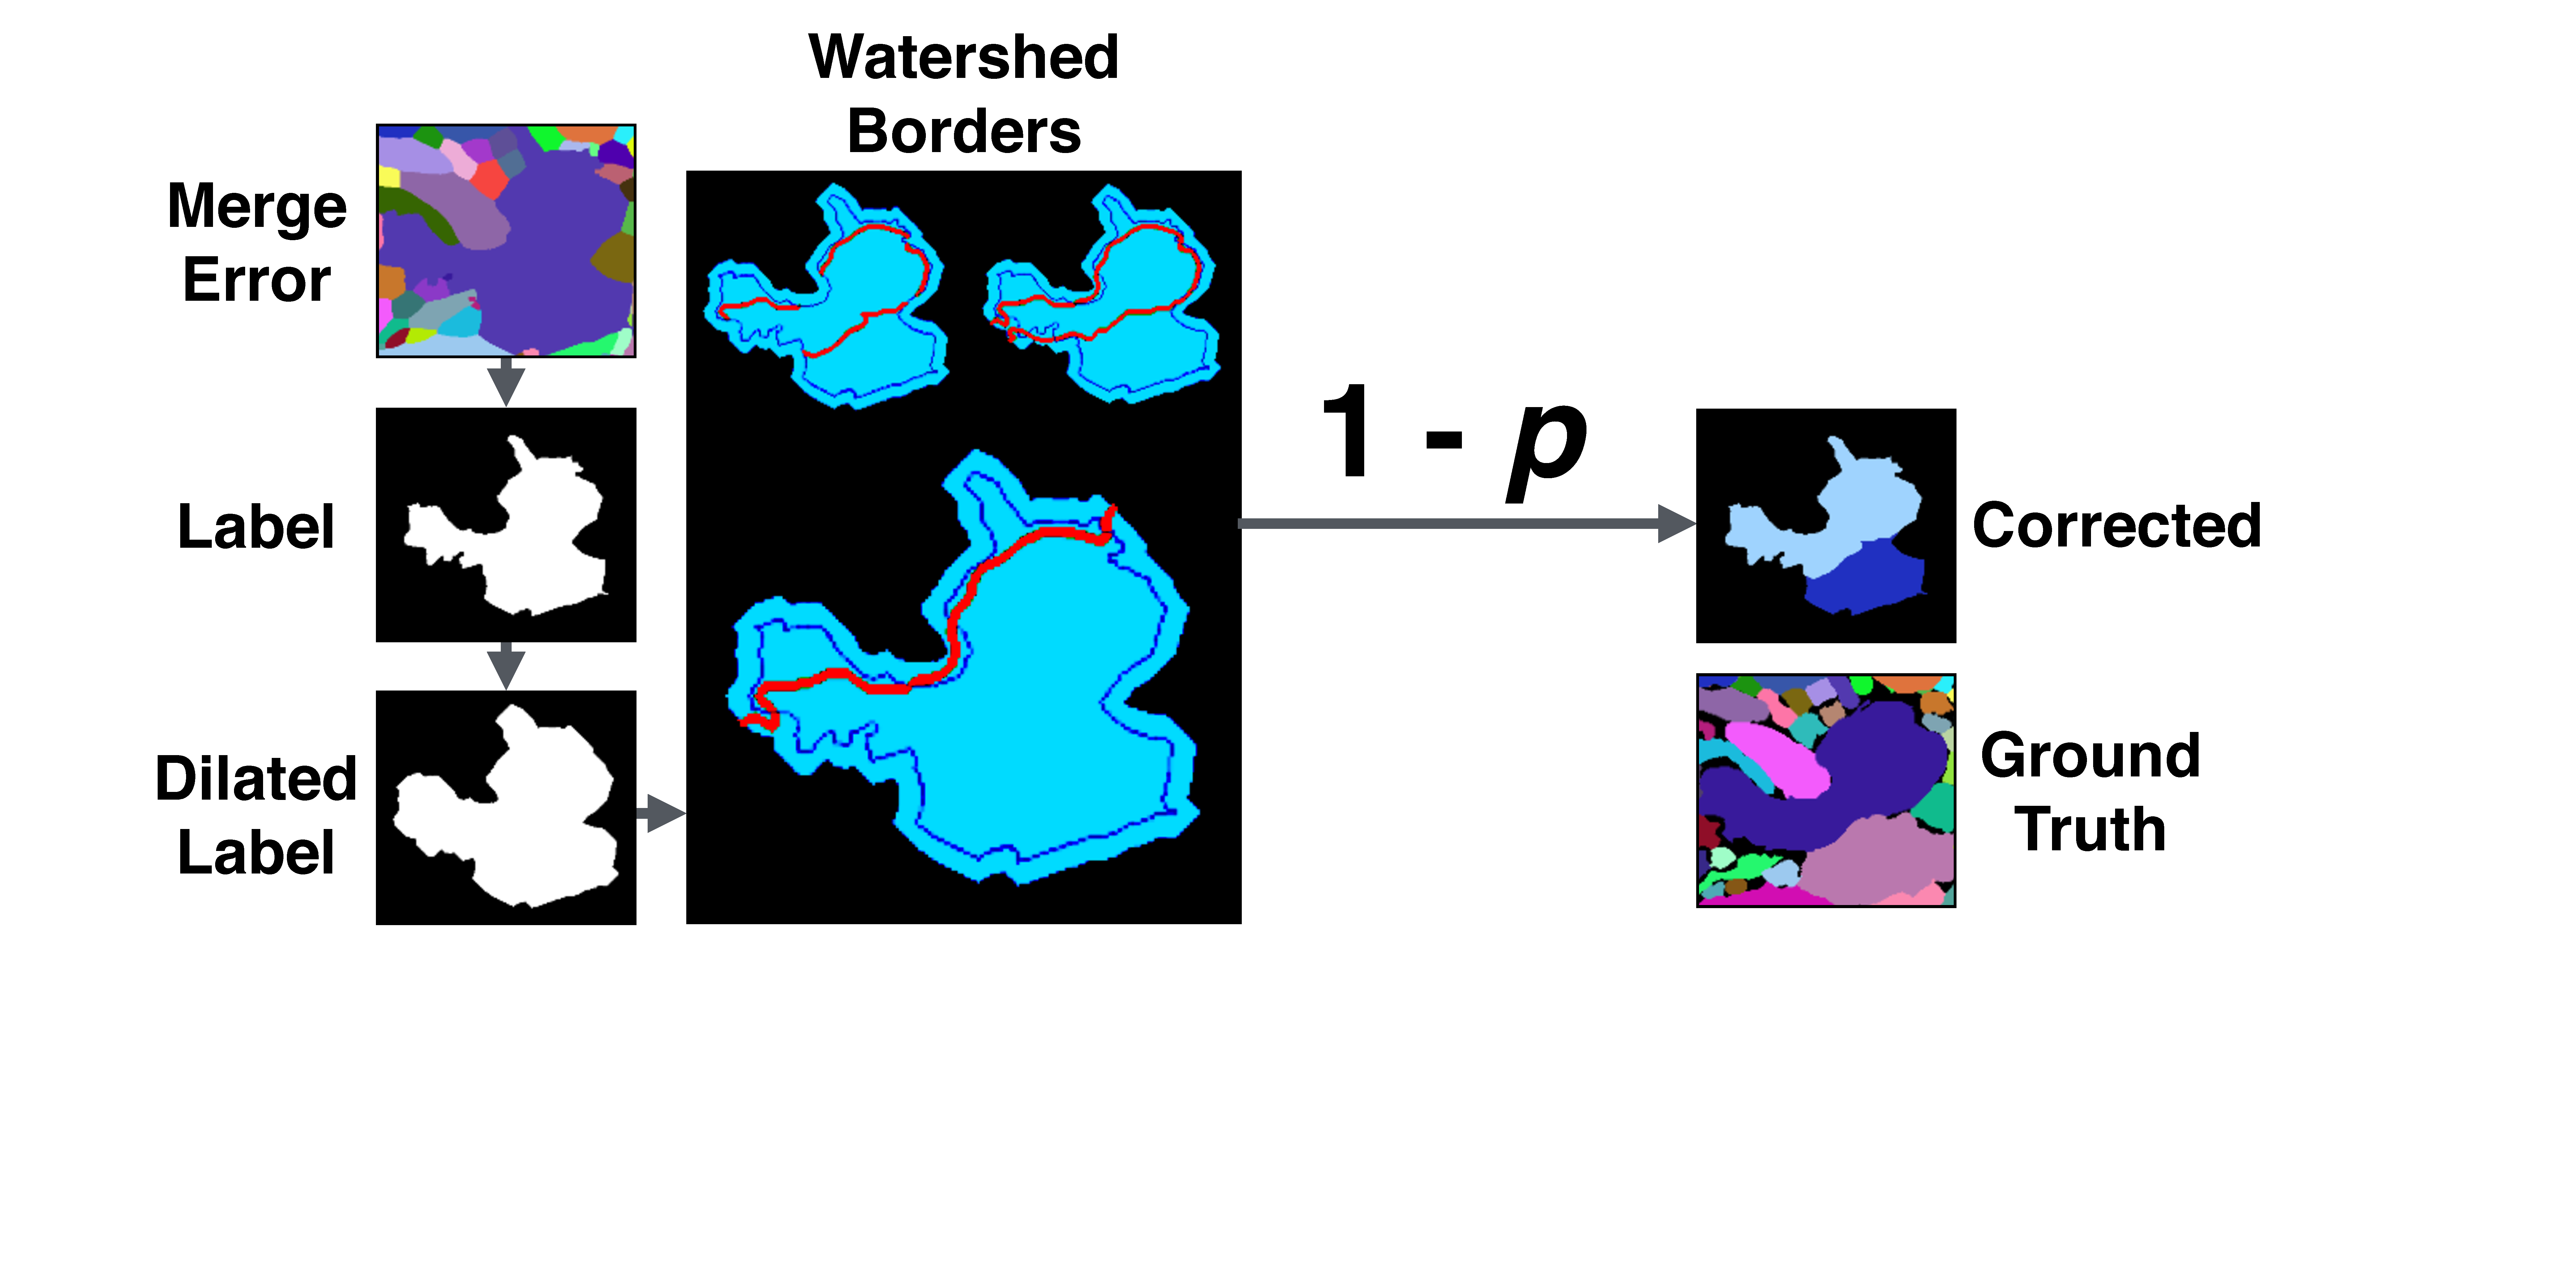
\includegraphics[width=\linewidth]{gfx/merge_error_v4.pdf}
\caption{Updated figure 4 to include the random watershed seeds. (TODO)}
\label{fig:merge_error}
\end{figure}


\section{GALA Active Learning Classifier}

We use GALA in our automatic segmentation pipeline (line 499). GALA uses a random forest classifier to agglomerate segments. While it does not require user interaction, it requires parameters. We will either add a reference to our yet unpublished segmentation pipeline or add a section to the supplemental material describing it in more detail as requested by reviewer 3.

%{\small
%\bibliographystyle{ieee}
%\bibliography{egbib}
%}

\end{document}
